\documentclass[12pt]{article}%
\usepackage{amsfonts}
\usepackage{fancyhdr}
\usepackage{comment}
\usepackage[a4paper, top=2.5cm, bottom=2.5cm, left=2.2cm, right=2.2cm]%
{geometry}
\usepackage{times}
\usepackage{amsmath}
\usepackage{changepage}
\usepackage{amssymb}
\usepackage{graphicx}%
\usepackage{lipsum}
\usepackage{array}
\usepackage{listings}
\usepackage{color}
\usepackage{xcolor}

\delimitershortfall-1sp
\newcommand\abs[1]{\left|#1\right|}
\graphicspath{ {./Images/} }

\definecolor{lightgray}{RGB}{214, 219, 223}
\definecolor{limegreen}{RGB}{11, 83, 69}
\definecolor{blue}{RGB}{0, 70, 255}
\lstdefinestyle{mystyle}{
    backgroundcolor=\color{lightgray},   
    commentstyle=\color{limegreen},
    keywordstyle=\color{blue},
    breaklines=true
}
 
\lstset{style=mystyle}
\makeatletter
\renewcommand{\maketitle}{\bgroup\setlength{\parindent}{0pt}
\begin{flushleft}
  \textbf{\@title}

  \@author
  \@date
\end{flushleft}\egroup
}
\makeatother


\begin{document}

\title{\large Course: CS3031 Advanced Telecommunications \\ \normalsize Title: Assignment 1 - Web Proxy Server Documentation}
\author{Name: Leong Kai Ler \\ Student Number: 15334636 \\   }
\date{Date: February 26, 2019}
\maketitle

\section*{Introduction:}
In computer networks, a proxy server is a server that acts as the intermediary application connecting the clients and servers. It is typically used to receive information seeking requests from clients and direct them towards the target servers. The functionalities of proxy servers also encompasses processes such as comprehending and evaluating complex requests before simplifying them. Furthermore, the implementation of proxy servers also adds layers of structure and encapsulation to distributed systems in real world. \\

\section*{Purpose:}
The purpose of this project is to design a web proxy sever that serves as a local server, in retrieving items from the Web on behalf of a Web client instead of the client fetching them directly. Such design enables the proxy server to control access flow through it and cache web pages. \\
\begin{center}
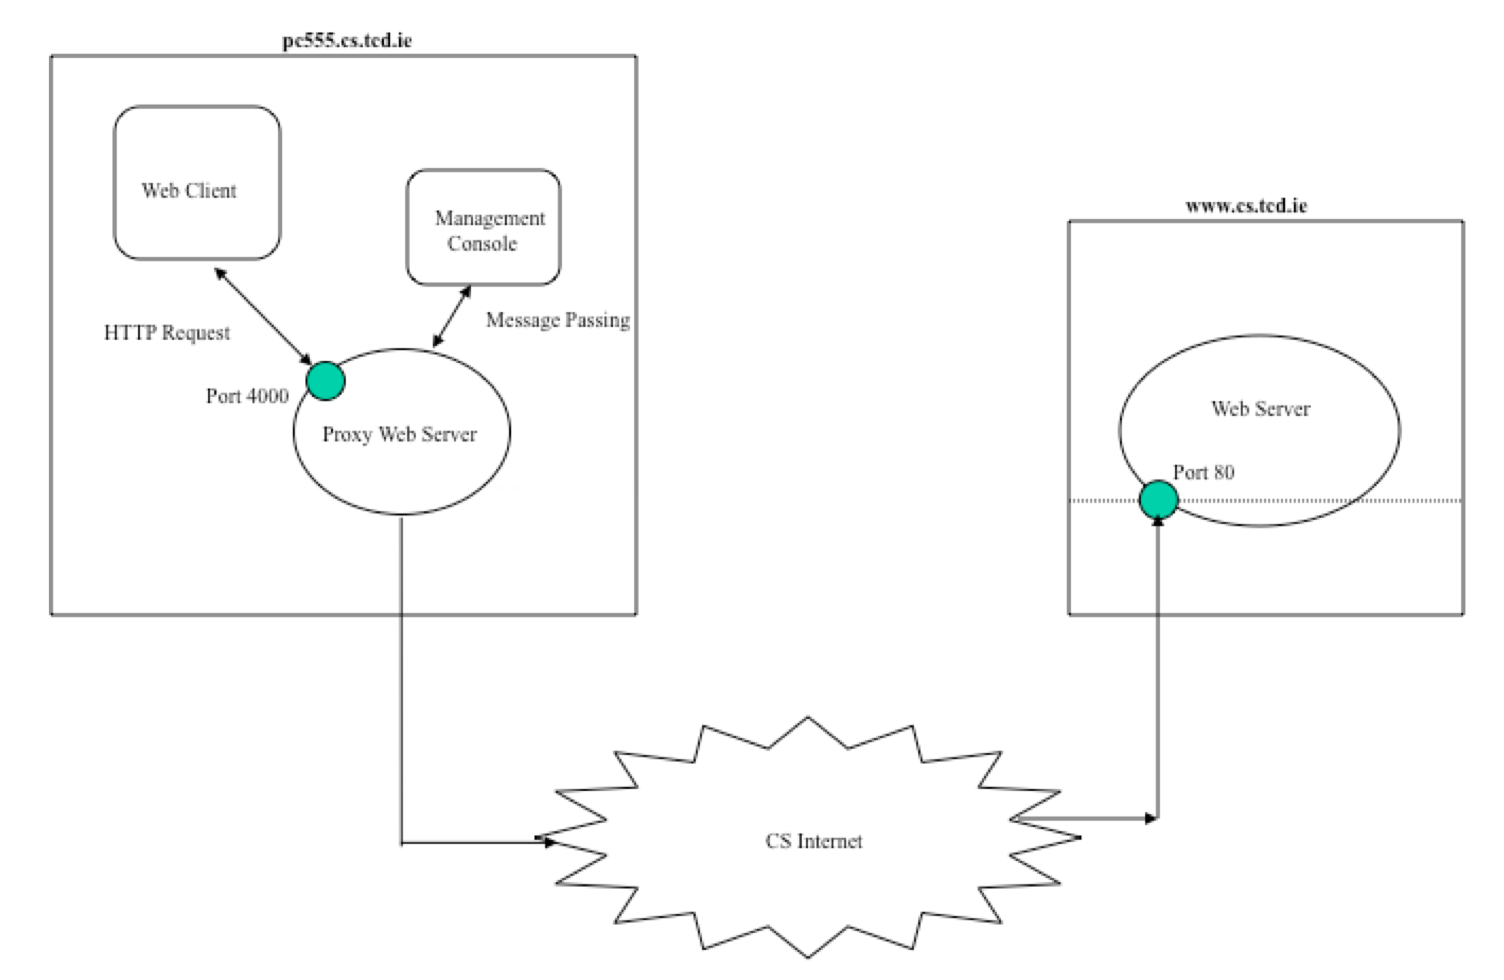
\includegraphics[scale=0.6]{designo}
\end{center}
\newpage
The functionalities of the web proxy server should include the following aspects:
\begin{itemize}
\item Respond to HTTP \& HTTPS requests, and should display each request on a management console. It should forward the request to the Web server and relay the response to the
browser. 
\item Handle websocket connections.
\item Dynamically block selected URLs via the management console.
\item Efficiently cache requests locally and thus save bandwidth. You must gather timing and bandwidth data to prove the efficiency of your proxy. 
\item Handle multiple requests simultaneously by implementing a threaded server.
\end{itemize}
\newpage
\section*{Design:}
As mentioned above the intended proxy server is divided into mainly two components: the web proxy server and a management console. This program is written using Java programming language.\\
\begin{center}
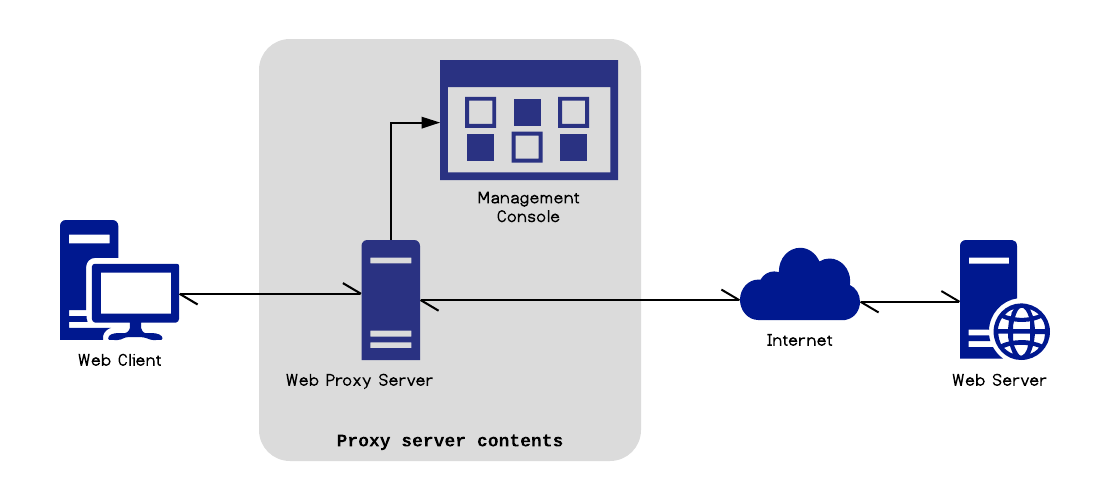
\includegraphics[scale=0.8]{design}
\end{center}
The management console is responsible in displaying the traffic on input and output of data streams through the proxy server, while the web proxy server listens to the web clients by creating threads and respond to their requests accordingly and setting up HTTP and HTTPS connections to retrieved information seek by web clients. It then relays the results of the request back to them respectively. A thread pool is created to access active threads each containing a request and execute them by creating sockets to establish connections between local server with web servers. In essence, the process of handling a HTTP request can be simplified as below: \\
\begin{center}
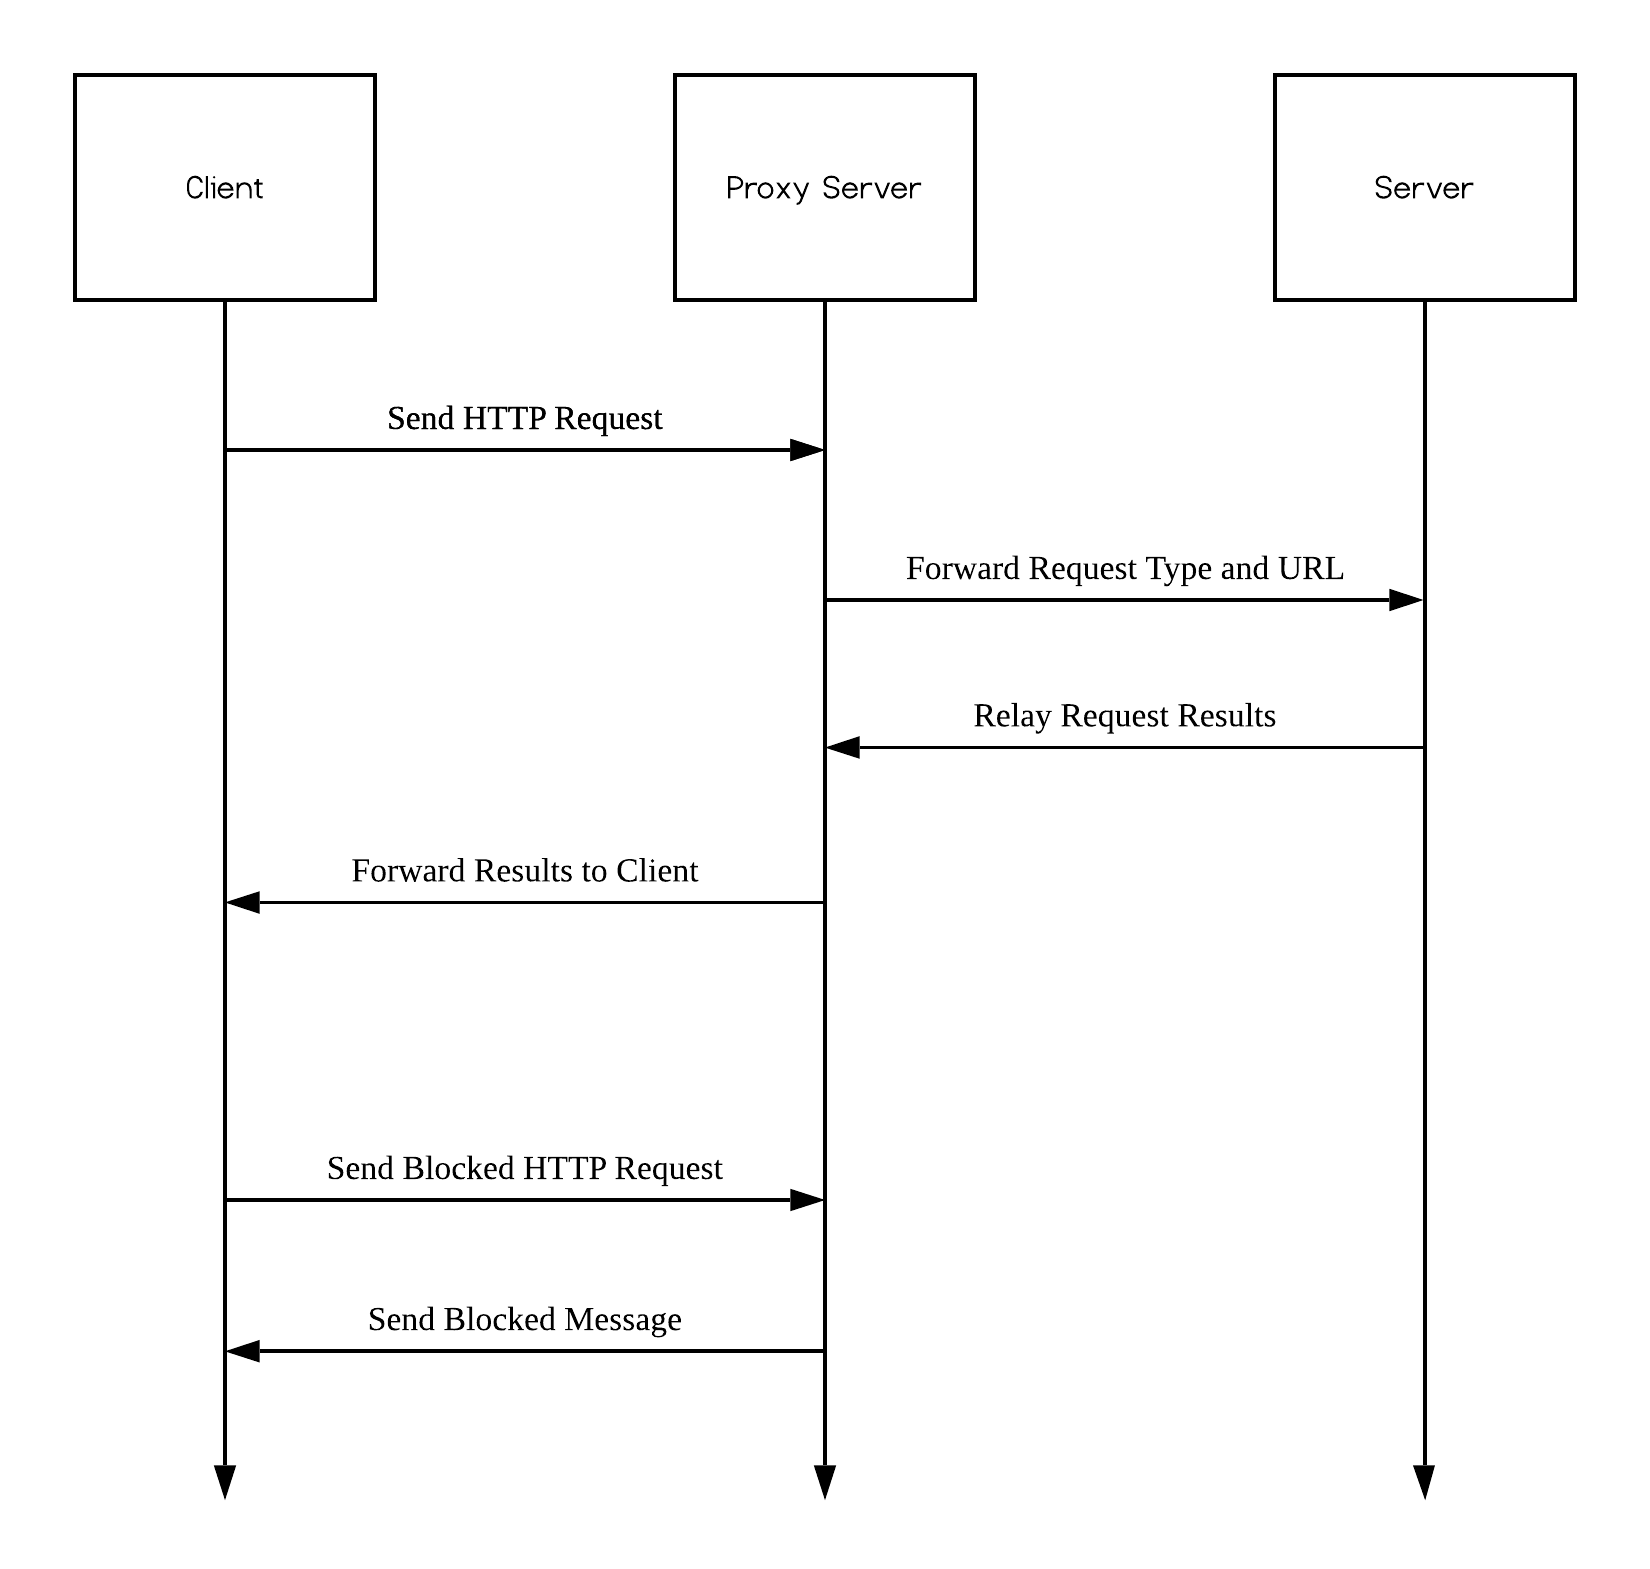
\includegraphics[scale=0.7]{http}
\end{center}
\newpage
On the other hand, the process of handling a HTTPS request would look slightly different as displayed in the following image:  
\begin{center}
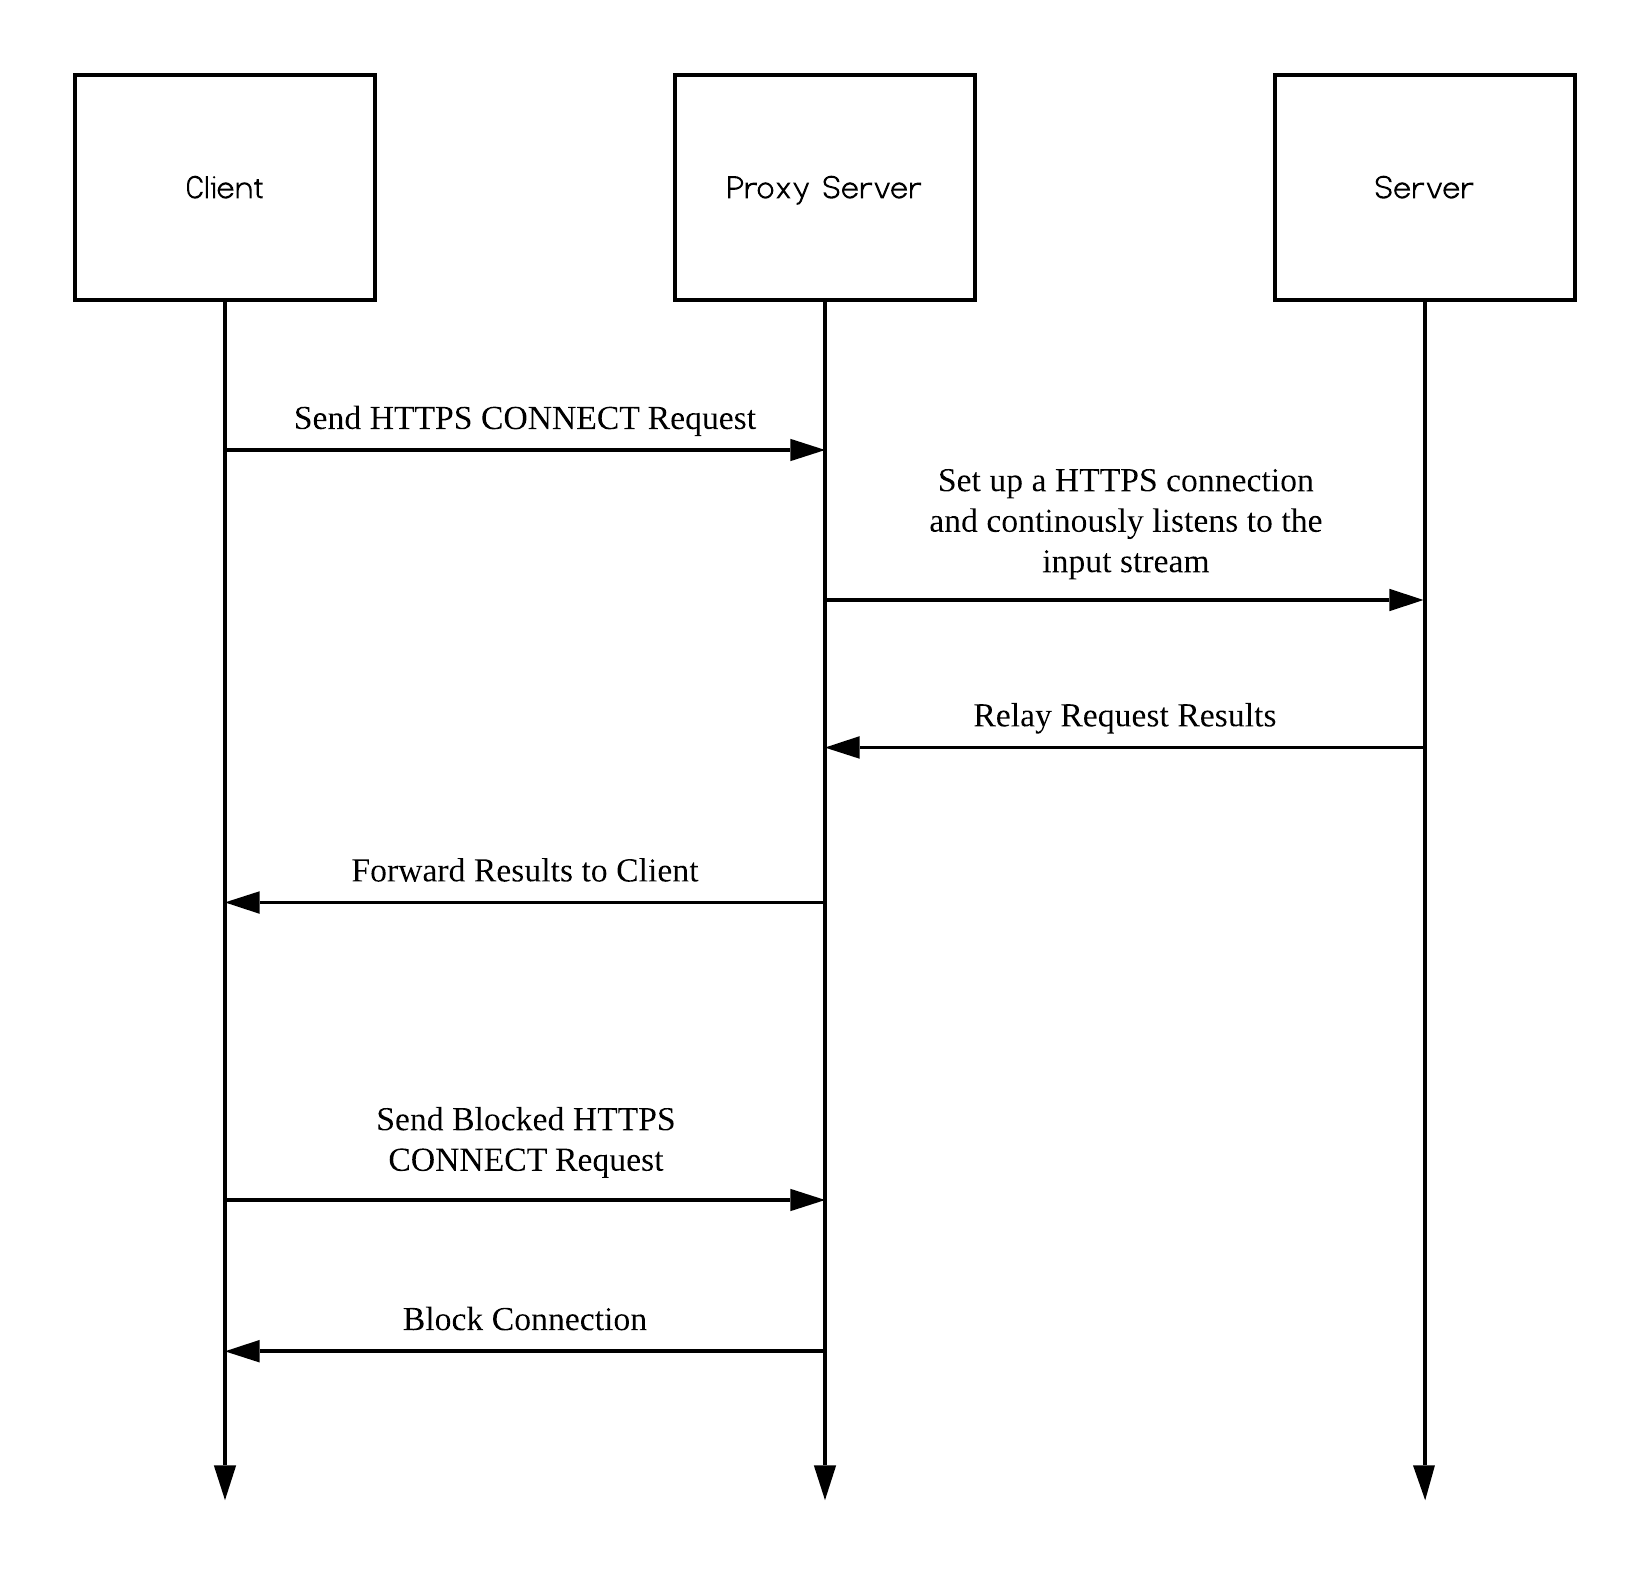
\includegraphics[scale=0.7]{http2}
\end{center}
Furthermore, it should be able to dynamically block websites that are stored in a blocked list. In other words, every time before setting up any connections, the proxy server has to confirm if the host names of the provided websites has been blacklisted. If the host name of the website is present in the blocked list, it should prevent the request from being executed and display a forbidden message as a warning signal to the web client. Otherwise, the web proxy can deal with the request normally. \\ \\
In order to improve operating efficiencies, a cache is to be set up to store data of previously visited websites. These data can range from normal text files, images in the form of png, jpg, jpeg or gif, html pages and etc. To achieve this, a hash map is set up to check for existence of a requested page in a cache set up before setting up a connection to deal with it. A timer has also been set up to display the difference in duration of handling GET request with and without the assistance of cache.  \\ \\
Additionally, every time when the proxy server is closed, the blocked website list and cached list has to be saved so that they are preserved the next time the proxy server is active. This can be done through serialization. Serialization is a data storage method that translates data structures or object state into a format by converting them into a stream of bytes so that they can be stored, transmitted and even reconstructed later. This allows us to preserve the state of the object when we recreate or de-serialize it the next time the proxy server is turned on.  \\ \\
Lastly, to enable web socket connections, the proxy server should be able to set up a special thread to handle HTTPS connections. To facilitate real-time data transfer to-and-from server due to interactions, this thread has to be able to take in continuous input stream of data from the web server socket, thus constructing a full-duplex communication between client and web server with the proxy server in between. \\

\newpage
\section*{Proxy Server:}
\subsection*{Flow chart:}
Overall, the flow of the proxy server operations as designed above can be visualized in a flow chart with countable states connected by several decision boxes: \\
\begin{center}
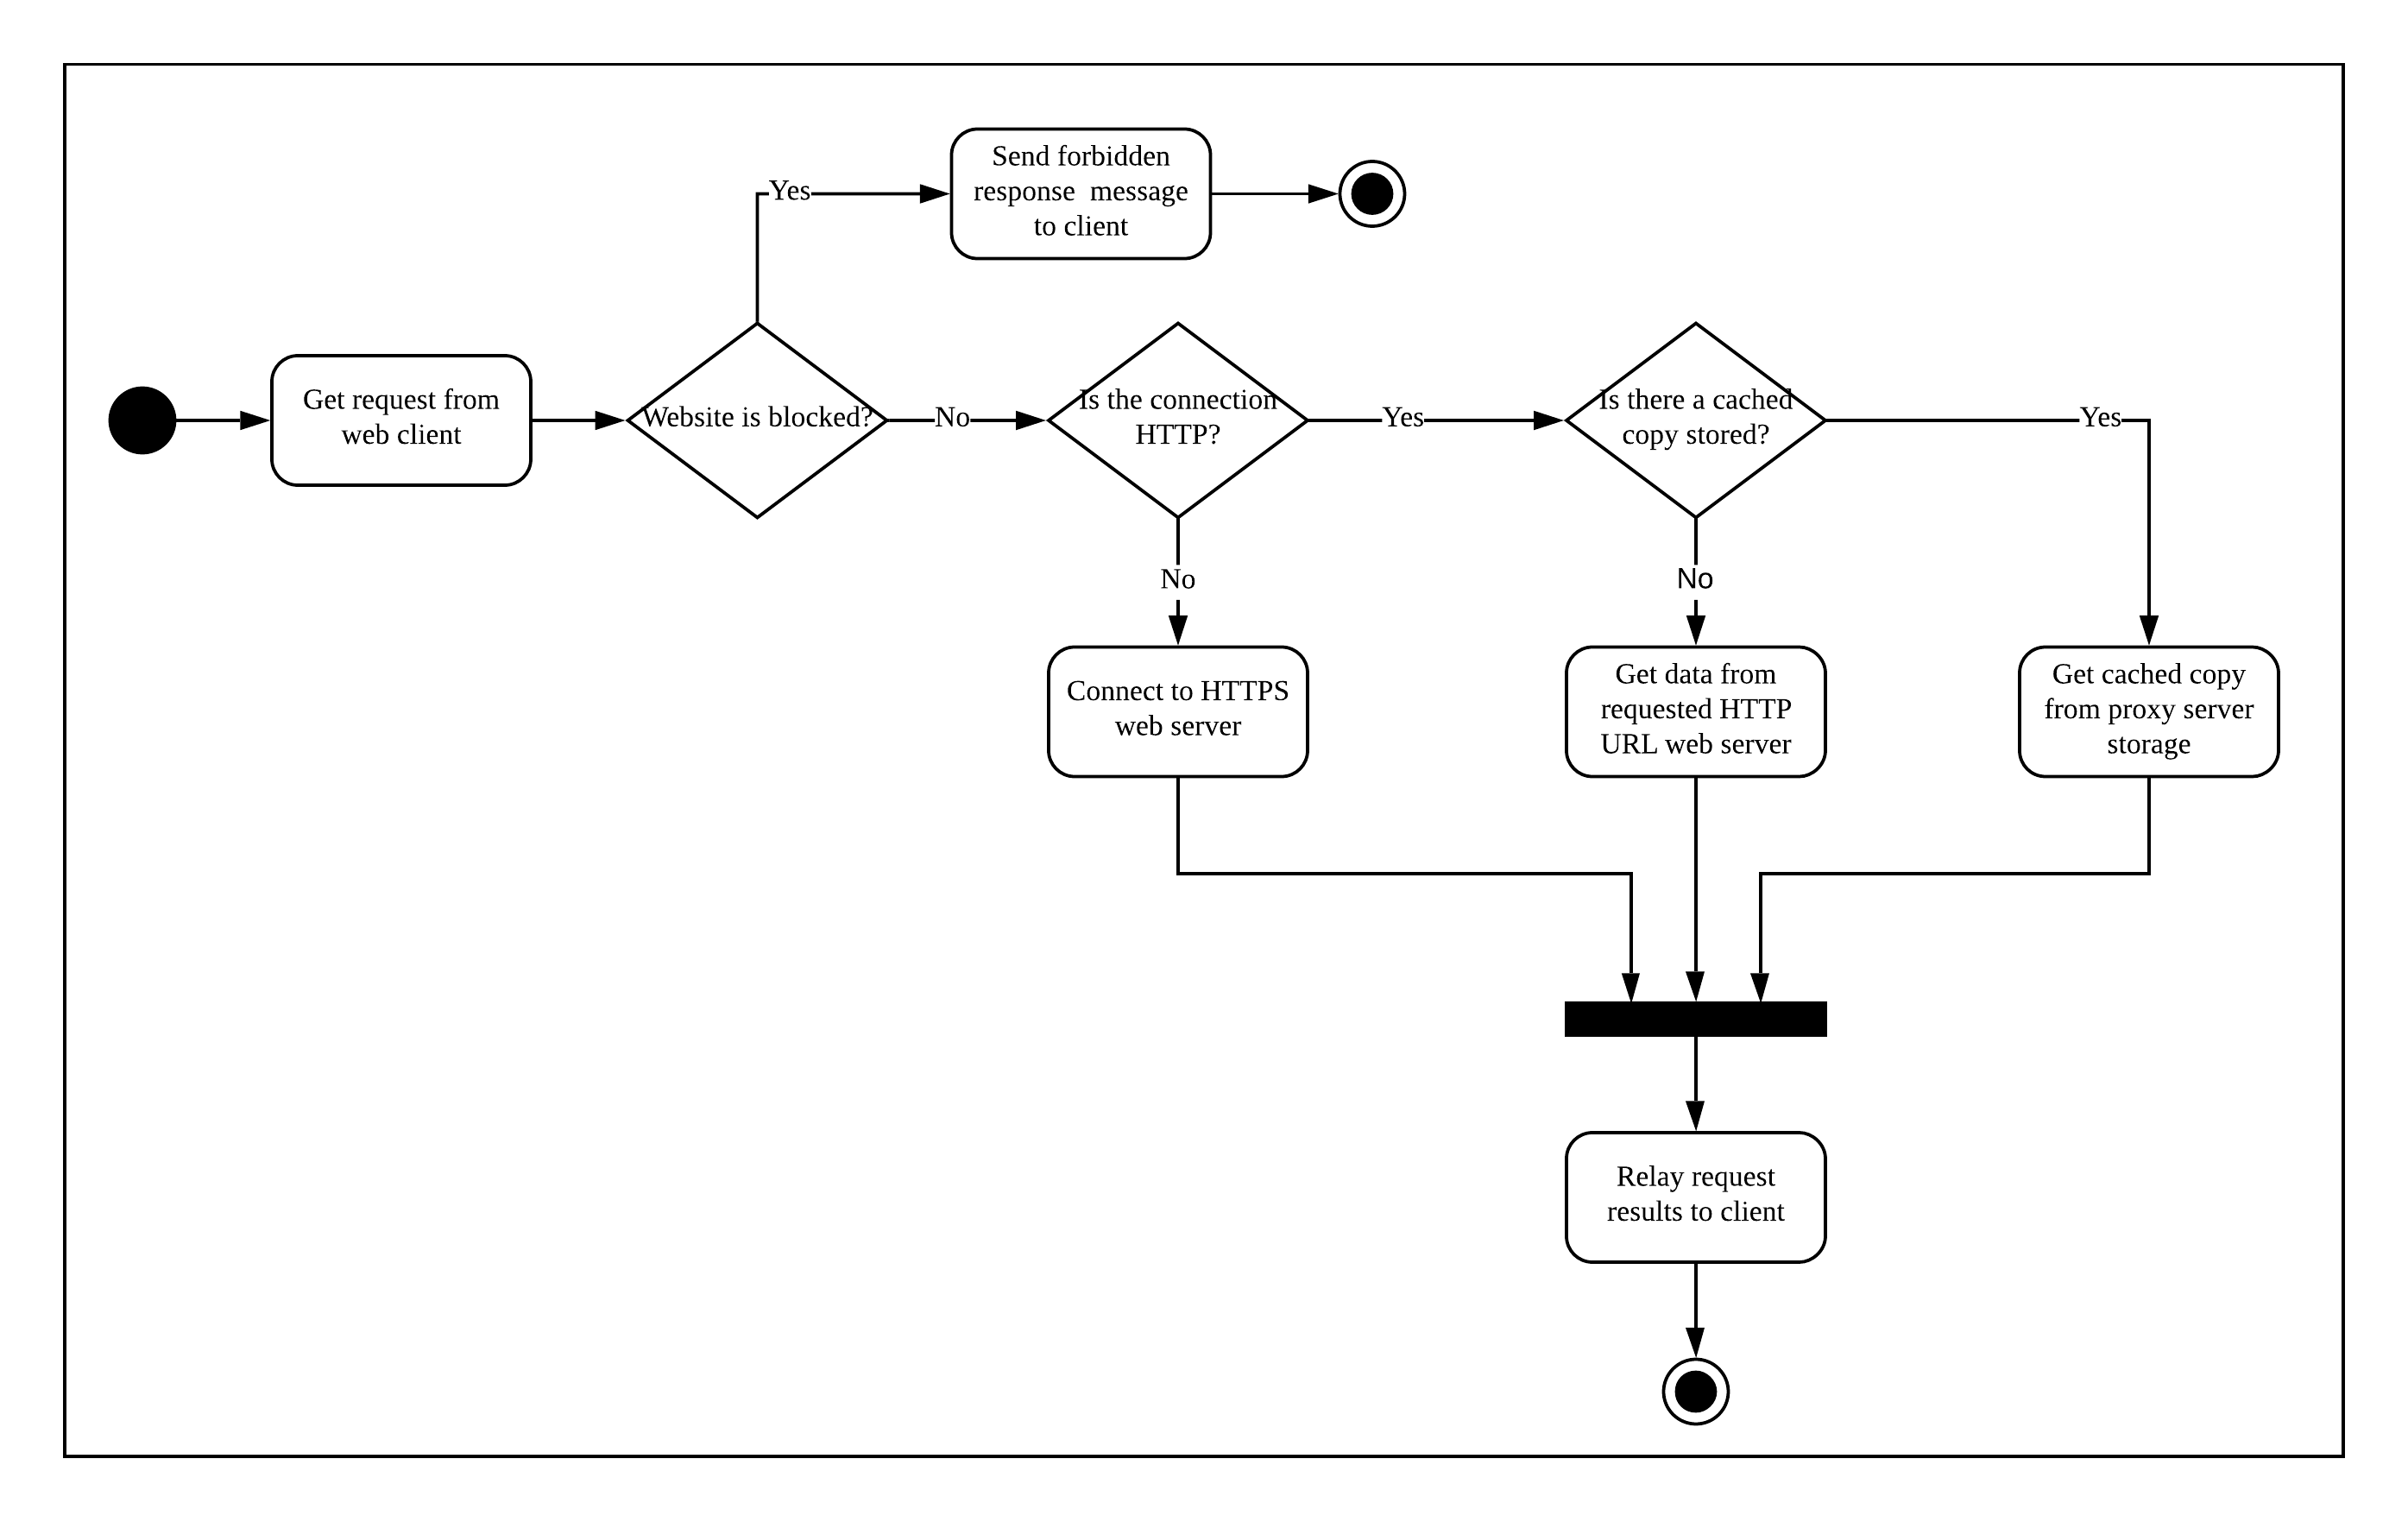
\includegraphics[scale=0.7]{flowchart}
\end{center}
In general, when a proxy server receives a request from web client, it will run through up to a maximum of 3 decision boxes to decide on its approach for the request based on its needs. But they will all in the end converge into one state, which is the proxy server relaying the results of the request to the web client, even if the message to be conveyed is an indication that the website requested is forbidden by the administrator. \\
\subsection*{Implementation:}
\subsection*{Setting up}
This program make extensive use of TCP sockets provided in Java.net.sockets library to handle connections. The proxy web server is implemented using server sockets that is capable of accepting multiple socket connections from clients and handles them simultaneously,thus allowing multi-threading. When the web proxy server socket receive a connection request from a client socket, it creates a thread to handle their request and the thread is then put into a thread pool for concurrent management during the process. Every time when the proxy web server is turned on, it will load back the cached data and blocked websites into their respective data structures, as a method of continuing its from previous state. \\ \\
To take in input request from and output messages as response to web clients and web servers, the proxy server make use of buffered readers and writers. Buffered Reader allows the web server to read lines of request and response from both sides and extract important information for further processing. On the other hand after the further processing, it will output the result of it using Buffered Writer, which is a versatile application in dealing with sending response code to sockets and writing data retrieved from socket output streams on a file. \\
\subsubsection*{Sending HTTP Request}
There two situations that can happened when dealing with HTTP request, that is if there is a cached copy available for the requested URL site or not. To deal with situation where there are no cached copies available typically during compulsory cache misses, the proxy server first creates a file using the url host name as the file name and the url extension as the file type extension. Then, depending on the type of requested data, whether if is an image or a text based page, the proxy server will set up http url connection to forward the GET request to the site and attempt to extract its data and relay it to the web client. At the same time, it will also try to save a copy of the visited site using a separate buffer writer or ImageIO if it is an image to store a copy of the result data into the file created earlier. The web cache is implemented using HashMap with the url as key and the file as its corresponding values, due to its resemblance to a normal cache, where the url act as the memory address and the file act as the data stored at that particular address. Suppose if the request was a failure, then a response code of 404 NOT FOUND will be transmitted to the client, otherwise a response code of HTTP 200 will be transmitted instead. HTTPUrlConnection is being prioritized over using sockets here due to its versatility to extract even the last modified date of a web page that can be used to implement the proper functionality of a web cache.\\ \\
Now, since there is a copy of the visited site preserved in the proxy server already, when the same site is being visited again, all that's needed to do is to find the file name of the saved copy in the cache using the url of the requested site as key to access the cache HashMap data structure. If there is hit, the contents of the file will be extracted using buffered reader and transmitted to client using buffered writer. This further reduces the time needed to transmit data as there's no need to set up a connection for retrieving data. \\
\subsubsection*{Sending HTTPS Request}
Sending a HTTPS request can be tricky. This is because HTTPS connections make use of secure sockets (SSL) making data transfer between clients and servers encrypted. To overcome this problem, the proxy server needs to know how to deal with the encrypted data. The approach used in this context is is called HTTP Tunneling method, which allow us to send encrypted data over public network. This is how it works. When the proxy server receives a CONNECT Request, it attempts to extract the destination url from the inputs and created a socket connection to the remote web server. A response code of 200 is sent to client as confirmation of the connection being established. Now all there's left id to create a thread that allows the continuous transmissions of data between client and server through the proxy server simultaneously, thus enabling web socket connections application. However, since the data input and output stream are encrypted, it will be difficult to cache the data. \\
\subsubsection*{Administrator:}
The proxy web server is set up in a way that only the administrator have the authority to manage its operation in real time. For example, the administrator has a higher privilege over the web clients, allowing him or her to block and unblock web pages. This allows him to have control access over data flowing in and out of the system, which is crucial to ensure the security of the proxy server. Moreover, the administrator can also shut down the web proxy server whenever he deems appropriate and thus terminating the request of the web clients to be served. \\
\subsubsection*{Blocking}
As mentioned, the administrator has the authority to block websites. This can be done by entering the URL of websites where the proxy server will convert them into host names and store them into a hash set. One reason that hash set is chosen as a data structure in this context is because that it prevents duplicates host names from being stored in the list, thus no extra memory space is being wasted on duplicate copies of blocked host names. \\ \\
Supposed a blocked website is being requested by a web client, instead of establishing a connection like the proxy server normally do, it will instead generate a forbidden access alert and output a denied access message to the web client, indicating that the requested website is blacklisted by the administrator due to security purposes. The forbidden response code would be 403. \\
\subsubsection*{Proxy Web Server shut down:}
As mentioned above that the proxy server maintains copies of previously cached data and blocked websites, so it is crucial that during the shut down of the proxy server socket, these files are being saved somehow beforehand. The initiative in this situation is by serializing them. This allow us to convert the cache hash map and blocked list hash set into stream of bytes that can be easily loaded back the next time the proxy server is turned on again. The files are then stored in a $.ser$ file and thus the state of the proxy server is somehow preserved for future use. Upon shutting down, all the threads in the thread pool will be terminated even though they have not finished executing and the server socket is also closed to avoid unmonitored and unwanted influx of data. \\
\subsection*{Code:}
\lstinputlisting[language=Java]{./java/ProxyServer.java}
\subsection*{Weakness:}
A flaw present in the system designed is that the cache implemented does not check if the copy supplied during HTTP request is the most updated version as present in the original web server. This causes potential wrong information to be supplied to web clients as the program only checks if the there is cached copy but not if it has been modified after the copy was first saved and stored in the data storage section. \\ \\
Moreover, a cache should operate in a way such that it stores only either the most recently or frequently accessed items depending on the proxy server needs. this is mainly due to the limited memory space it has. Therefore, the implementation of cache using only a Hash Map is obviously not an appropriate choice here because there is no way to trace for data that haven't been accessed for a long time and seek to remove them in order to clear up space in the cache. \\
\subsection*{Improvements:}
To solve the problems above, we can formulate alternatives that are specifically designed to tackle each of them. Firstly, by using the library class HttpURLConnection as provided in Java programming language, it allows us to extract various information such as host names, response code, certificates, and even last modified date of a web page. Utilizing this advantage, we can propose checks that set up a url connection to the requested website when a cached copy is requested. This allow us to compare the last modified date retrieved and the current modified date stored along with the files to ensure the validity of our copy. If the copy possessed is out of date, then the proxy server simply fetches a new one and display it to the client and as well as renewing its copy. That being said the file copy should now be stored in a wrapper class along with the last modified date for easier access. \\ \\
Moreover, in order to properly simulate the operations of a cache, a Least Recently Used(LRU) queue class can be implemented to overcome the shortcomings of Hash Map in this context. A queue can be set to a limit size to prevent excess data from being stored on the proxy server, which could be detrimental to its processing speed. At any point, when the limit size is exceeded, the cache will begin dequeuing data on the head to clear up space for incoming data.
\newpage
\section*{Request Handler(Management Console in code due to naming error): }
\subsection*{Implementation:}
\subsubsection*{Request Handler}
The Request Handler is implemented to take in request from web clients and handles them properly based on types of request such as GET and CONNECT. \\
\subsubsection*{Management Console}
The management console in the form of a printer associated with operations of the proxy server, allowing it to print out all the traffic data of each execution of threads' requests. 
\subsection*{Code:}
\lstinputlisting[language=Java]{./java/ManagementConsole.java}
\subsection*{Weakness:}
The traffic data displayed on Request Handler can only be differentiated between normal data and exceptions raised. This makes debugging abnormal problems difficult as there are way too many data flowing through the proxy web server in a continuous stream. 
\subsection*{Improvements:}
One approach in dealing with such situations is to assigned different color codes to threads based on their request execution conditions. The colors will represent the status and state of the request being executed  and indicate whether the result returned is positive or not using ratings. Such method will save more time for testers to figure out which request generated is facing problems and be sorted out early to avoid congestion in the traffic data pool. 
\end{document}